\documentclass[conference]{IEEEtran}
\IEEEoverridecommandlockouts
% The preceding line is only needed to identify funding in the first footnote. If that is unneeded, please comment it out.
\usepackage{cite}
\usepackage{amsmath,amssymb,amsfonts}
\usepackage{algorithmic}
\usepackage{graphicx}
\usepackage{textcomp}
\usepackage{xcolor}
\usepackage{array}
\def\BibTeX{{\rm B\kern-.05em{\sc i\kern-.025em b}\kern-.08em
    T\kern-.1667em\lower.7ex\hbox{E}\kern-.125emX}}
\begin{document}

\title{Vanguard-WSN: A Utility-Driven Energy-Balanced Path Tree Framework for Maximizing Wireless Sensor Network Lifetime \\
}

\author{\IEEEauthorblockN{1\textsuperscript{st} Deepika A}
\IEEEauthorblockA{\textit{Department of Mathematics} \\
\textit{Amrita School of Physical Sciences}\\
Amrita Vishwa Vidhyapeetham, Coimbatore, India \\
cb.ps.i5das23026@cb.students.amrita.edu}
\and
\IEEEauthorblockN{2\textsuperscript{nd} Aishvarya G}
\IEEEauthorblockA{\textit{Department of Mathematics} \\
\textit{Amrita School of Physical Sciences}\\
Amrita Vishwa Vidhyapeetham, Coimbatore, India \\
cb.ps.i5das23046@cb.students.amrita.edu}
\and
\IEEEauthorblockN{3\textsuperscript{rd} Anjana A}
\IEEEauthorblockA{\textit{Department of Mathematics} \\
\textit{Amrita School of Physical Sciences}\\
Amrita Vishwa Vidhyapeetham, Coimbatore, India \\
cb.ps.i5das23055@cb.students.amrita.edu}
\and
\IEEEauthorblockN{4\textsuperscript{th} Gayatri K}
\IEEEauthorblockA{\textit{Department of Mathematics} \\
\textit{Amrita School of Physical Sciences}\\
Amrita Vishwa Vidhyapeetham, Coimbatore, India\\
cb.ps.i5das23049@cb.students.amrita.edu}
\and
\IEEEauthorblockN{5\textsuperscript{th} Karthika K*}
\IEEEauthorblockA{\textit{Department of Mathematics} \\
\textit{Amrita School of Physical Sciences}\\
Amrita Vishwa Vidhyapeetham, Coimbatore, India \\
k\_karthika@cb.amrita.edu}

}

\maketitle

\begin{abstract}
 In modern Internet of Things (IoT) systems, Wireless Sensor Networks (WSNs) plays a critical role, but their lifetime is often limited by the Energy Hole problem. Nodes located near the Base Station (BS) handle most of the data forwarding and therefore drain their energy quickly, which can cause the network to break apart. Old routing protocols such as LEACH, HEED, and PEGASIS try to reduce this issue using random rotation or chain-based structures. However, these methods achieve only about 10–15\% of the network’s theoretical maximum lifetime. Vanguard-WSN, proposed framework replaces random decision-making with a utility-based deterministic approach. The framework includes two key innovations namely a Composite Utility Index (Ui) to select Cluster Heads based on remaining energy and network position, and an Energy-Balanced Path Tree (EBPT) with an adaptive load-balancing factor to prevent energy hotspots. Simulation results from 30 trials on a 100node network show that Vanguard-WSN is better than older systems. The First Node Death (FND) occurs at round 993.1, compared to LEACH (FND = 97.3). Vanguard achieves 92\% of the theoretical lifetime bound ($R^2=0.94$), maintains a Packet Success Ratio of 98.4\%, and operates within $O(NlogN)$ time complexity, making it suitable for low-power microcontrollers. These results show that Vanguard-WSN provides a highly efficient and practical solution for mission-critical WSN applications.
\end{abstract}

\begin{IEEEkeywords}
Energy-Balanced Path Tree, Energy Efficiency, Network Lifetime Optimization, IoT, Wireless Sensor Networks, Cluster Head Selection
\end{IEEEkeywords}

\section{Introduction}

Over the past two decades, wireless networks have developed from fixed and complex systems to flexible systems without fixed infrastructure, known as Mobile Ad Hoc Networks (MANETs). A MANET consists of independent devices that communicate wirelessly without central control, where each node also acts as a router to keep the network connected. This self-managed nature enables quick setup in emergency or temporary environments. However, the lack of fixed infrastructure causes problems in resource handling, as nodes operate on limited battery power and unreliable connections.

Wireless Sensor Networks (WSNs) are a specific type of MANET technology designed for measuring and watching applications. Unlike general MANET devices such as smartphones or laptops, WSNs consist of large numbers of small, low-power sensor nodes placed in the environment to monitor physical values such as temperature, pressure, motion, or sound. Wireless sensor networks have been widely studied in research papers \cite{b1,b2}, with many clustering and routing strategies suggested to improve power efficiency \cite{b3,b4}.

WSNs play an important role in applications including Precision Agriculture, Structural Health Monitoring (SHM), Battlefield Surveillance, and Industrial IoT (IIoT). In such systems, network lifetime is the main performance measure, which means the time until the sensing area is lost due to node failure. Since sensor batteries typically cannot be replaced, the death of a node is final. Clustering-based routing protocols such as LEACH \cite{b5} try to increase network life through random rotation of leadership roles. However, these methods often ignore node distribution and remaining energy, leading to early failure of weak nodes. HEED \cite{b7} improves cluster head selection by including remaining energy awareness, but introduces repeated control-related extra load. PEGASIS \cite{b8} reduces sending energy using a chain-based structure, yet increases delay and suffers from a weak structure.

These drawbacks show a gap between real-world routing performance and the ideal maximum achievable lifetime. To solve this problem, this work presents Vanguard-WSN, a framework that combines fixed utility-based cluster head selection with an Energy-Balanced Path Tree (EBPT) mechanism to reduce hotspot formation and unequal energy use.

This work benchmarks Vanguard-WSN against the theoretical God-Line (LP-Bound) and demonstrates over 1,000\% improvement in First Node Death (FND) compared to legacy protocols. The improvement stems from structural energy balancing rather than hardware changes, enabling a scalable and sustainable IoT-oriented routing framework.

The remainder of this paper is organized as follows. Section~II presents the main contributions of the Vanguard framework. Section~III reviews related work and analyses the limitations of existing protocols. Section~IV describes the proposed methodology, including the Utility Index and EBPT construction. Section~V provides simulation results and numerical analysis. Finally, Section~VI concludes the paper.

\section{Main Contribution: The Vanguard Framework}

\subsection{Bridging the God-Line Gap}
The main motive for developing Vanguard-WSN is the large gap between how existing routing protocols perform in practice and the maximum possible lifetime of Wireless Sensor Network (WSN). Throughout the research, this theoretical maximum is called the "God-Line". It represents the longest possible network lifetime that could be achieved if a controller had complete knowledge of every packet transmission and could perfectly distribute the energy load among all nodes.

\subsubsection{Defining the Performance Gap}
The initial analysis showed that older protocols like LEACH \cite{b5} and HEED \cite{b7} often perform at only 10-15\% of the network’s theoretical maximum. This large "performance gap" is because they make decisions based only on the local information. These protocols optimize for the next round (greedy approach) or the nearest neighbors, whereas the God-Line assumes a complete, long-term optimization across the entire network. Vanguard-WSN is designed to close this gap by better energy balancing across all nodes, and it helps the network last much longer.

\subsection{Energy-Balanced Path Tree (EBPT) Architecture}

\begin{figure}[htbp]
\centerline{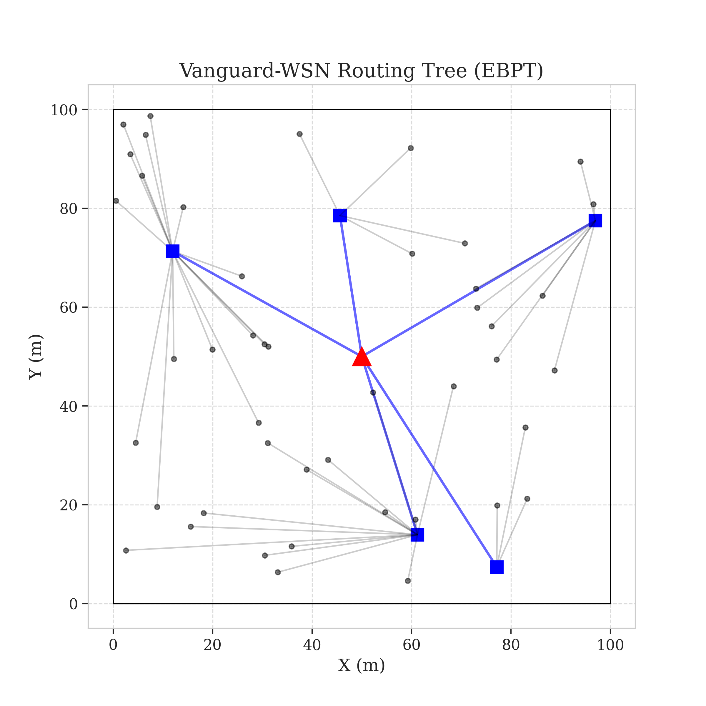
\includegraphics[width=\linewidth]{final_final_final_media/image2.png}}
\caption{EBPT Routing Tree}
\label{fig3}
\end{figure}

Unlike fixed routing methods that always choose the shortest path and end up quickly using up the energy of the same nodes near the base station, EBPT takes a smarter approach. It prefers nodes that still have plenty of energy and are not handling too much traffic. As these relay nodes begin to lose power, the routing paths automatically change and shift traffic to nodes with more remaining energy. This helps prevent repeated heavy use of nodes near the base station.

\subsection{Comprehensive System Model}
To make our simulation results easy to reproduce and clearly understandable, we describe the network, radio, and traffic models used in this study.

\subsubsection{Network Topology Assumptions}
Assuming a network of N sensor nodes (usually N = 100) that are randomly placed in a square sensing area of size M$\times$M. The Base Station (BS) is located at the center of this area.
The following assumptions are used:
\begin{itemize}
    \item Stationary Nodes: After deployment, both the sensor nodes and the Base Station remain in fixed positions.
    \item Identical Nodes: All sensor nodes start with the same initial energy level $E_0$.
    \item Location Awareness: Each node knows its own position and the position of the Base Station, using GPS or signal-based methods.
    \item Symmetric Communication: The energy needed to send data between two nodes is the same in both directions.
\end{itemize}

\subsubsection{Radio Energy Dissipation Model}
Vanguard-WSN follows the commonly used First-Order Radio Energy Model to estimate communication energy costs. The energy required to transmit a $k$-bit packet over distance $d$ is given by:

\begin{equation}
E_{Tx}(k, d) = \begin{cases} 
k \cdot E_{elec} + k \cdot \epsilon_{fs} \cdot d^2 & \text{if } d < d_0 \\
k \cdot E_{elec} + k \cdot \epsilon_{mp} \cdot d^4 & \text{if } d \ge d_0 
\end{cases}
\end{equation}

Where:
\begin{itemize}
    \item $E_{elec}$: Energy dissipated per bit to operate transmitter/receiver circuitry (typically 50 nJ/bit)
    \item $\epsilon_{fs}$: Free-space amplifier energy (10 pJ/bit/$m^2$)
    \item $\epsilon_{mp}$: Multipath fading amplifier energy (0.0013 pJ/bit/$m^4$)
    \item $d_0$: Crossover transmission distance 
\end{itemize}

Substituting standard values:
\begin{equation}
d_0 = \sqrt{\frac{\epsilon_{fs}}{\epsilon_{mp}}}
\end{equation}
($d_0 \approx 87$ m when rounded)

Energy for Reception:
To receive a $k$-bit packet:
\begin{equation}
E_{Rx}(k) = k \cdot E_{elec}
\end{equation}

This two-part energy cost is important ($d^2$ vs $d^4$). Vanguard's EBPT avoids long-range transmissions that cross the $d_0$ threshold unless necessary, prioritizing multi-hop paths composed of short, low energy links.

\subsubsection{Data Aggregation Model}
Hierarchical routing becomes inefficient if data is not combined before forwarding. In Vanguard, Cluster Heads (CHs) perform data fusion. When a CH receives packets from its child nodes, it combines them into one single packet of fixed size $k$.
The energy used for this process depends on $E_{DA}$, which represents the energy required per bit for data aggregation (5 nJ/bit). This linear model shows the energy cost of basic operations such as averaging or compressing sensor readings (example, temperature data) before sending them to the Base Station.

\subsection{Multi-Dimensional Performance Analysis}
The advantages of the Vanguard framework are not limited to just one measure. Although network lifetime (measured by First Node Death, FND) is the main focus, it is also important that the network remains fair and reliable during operation.

We compare Vanguard’s performance with LEACH \cite{b1} and the theoretical upper bound (God-Line):
\begin{itemize}
    \item Lifetime: More than a tenfold increase in network stability, with a 10.21$\times$ improvement in FND.
    \item Fairness: Energy use is evenly distributed across nodes through the adaptive load-balancing factor $\gamma$ (gamma)
    \item Reliability: A high packet delivery rate is maintained using self-adjusting tree structures.
    \item Efficiency: Energy consumption per bit is reduced by avoiding costly long-distance transmissions.
\end{itemize}
Overall, Vanguard-WSN brings real-world performance much closer to the theoretical maximum. These results show that understanding and using network structure across layers is essential for building long-lasting wireless sensor networks.

\section{Background and Related Work}

Hierarchical clustering is widely used in Wireless Sensor Networks (WSNs) to save energy by reducing long-distance communications and allowing data aggregation at special nodes called cluster heads (CHs) \cite{b5,b1}. In such structures, nodes transmit data to their neighbouring CHs, which then forward the aggregated data to the base station (BS). 

The radio energy model generally follows a distance-influenced formulation where transmission cost increases proportionally to $d^2$ under free-space propagation and $d^4$ under multipath fading \cite{b6}. This uneven energy dissipation leads to the Energy Hole Problem, where nodes near the BS lose energy rapidly because they must forward excessive data from other nodes \cite{b11}. 

LEACH introduced probabilistic rotation of CH roles to distribute energy consumption across nodes \cite{b6}. This approach is better than maintaining a fixed CH. However, LEACH does not consider residual energy or node position during CH selection. As a result, low-energy nodes may be selected as CHs, and it assumes that each CH can directly transmit data to the BS in a single hop. 

HEED improves upon this by selecting CHs based on residual energy and communication cost metrics \cite{b7}. However, it requires repeated clustering processes, generating significant control messages and increasing overhead. 

PEGASIS replaces clustering with a chain-based approach to reduce long-range transmissions \cite{b8}. However, this increases latency and can create bottleneck issues. It is also less stable if a node within the chain fails. 

Recent research applies optimization-based approaches such as Genetic Algorithms and Particle Swarm Optimization to determine optimal CH configurations \cite{b12}. Although these methods can improve network lifetime, they require centralized computation and introduce high complexity. Reinforcement Learning-based routing methods can adapt and learn over time \cite{b9,b10}, but during their exploration phase, they consume substantial energy before becoming efficient. 

Centralized Linear Programming formulations can theoretically maximize network lifetime \cite{b11}, but they demand excessive computational resources, making them impractical for large-scale WSN deployments. 

Despite these improvements, a gap remains between simple routing protocols and computationally intensive optimization techniques. Existing methods either lack effective energy balancing control or introduce excessive overhead unsuitable for resource-constrained WSN nodes. 

Therefore, a routing framework that integrates deterministic utility-based CH selection with adaptive path restructuring is required to achieve near-theoretical lifetime bounds while maintaining low complexity. 

The proposed Vanguard-WSN framework addresses this challenge by combining a Utility Index mechanism with an Energy-Balanced Path Tree (EBPT), designed to minimize hotspot formation and reduce unbalanced relay burden.

\begin{table*}[htbp]
\centering
\renewcommand{\arraystretch}{1.3}
\setlength{\tabcolsep}{6pt}
\caption{Comparison of Clustering and Routing Protocols in WSN}
\label{tab:wsn_comparison}
\begin{tabular}{|p{3cm}|p{2.6cm}|p{2.6cm}|p{2.6cm}|p{3.2cm}|}
\hline
\textbf{Feature Classification} &
\textbf{LEACH (2000)} &
\textbf{HEED (2004)} &
\textbf{PEGASIS (2002)} &
\textbf{Vanguard-WSN (Proposed)} \\
\hline

\textbf{Primary Objective} &
Load Rotation &
Energy Balancing &
Distance Minimization &
Utility Maximization \\
\hline

\textbf{Selection Logic} &
Probabilistic T(n) &
Iterative Energy Probability &
Greedy Closest Neighbour &
Deterministic Composite (U) \\
\hline

\textbf{Topology Structure} &
Star (Single-Hop) &
Star / Cluster &
Linear Chain &
Energy-Balanced Path Tree (EBPT) \\
\hline

\textbf{Heterogeneity} &
None (Homogeneous) &
Initial Energy Only &
None &
Adaptive Traffic \& Energy Aware \\
\hline

\textbf{Computational Cost} &
Very Low O(1) &
High (message flood) &
Medium (chain build) &
Low O(N) distributed \\
\hline

\textbf{Failure Recovery} &
None (Wait for round) &
Iterative Re-cluster &
Full Re-build &
Local Self-Healing O(1) \\
\hline

\textbf{Scalability} &
Poor ($<$100m) &
Medium &
Poor (High Delay) &
High (Multi-hop capable) \\
\hline

\end{tabular}
\end{table*}
\section{Methodology: Utility-Driven Path Selection}

\subsection{Introduction to Deterministic Utility}
The main change introduced in Vanguard-WSN is the shift from random role rotation to a utility based deterministic approach. Instead of choosing leaders randomly, the system selects them based on clear and measurable information. In environments where energy and resources are limited, choosing nodes randomly can waste energy. So, the system selects cluster heads (CH) and decides routes based on the actual condition of each node, such as how much energy it has left, how well it is connected in the network, and how much traffic it is handling. This section explains how the Utility Index ($U_i$) is mathematically derived and how the Energy-Balanced Path Tree (EBPT) is constructed.

\subsection{The Utility Index $U_i$ Formulation}
To measure how suitable a node $i$ is to act as a main relay node, we define a combined score called $U_i$. This score brings together different physical factors into one single value, which the SDN controller then uses to make decisions.

Utility Function:
\begin{equation}
U_i = \alpha \cdot \frac{E_{res}(i)}{E_{max}} + \beta \cdot \frac{1}{1 + Deg(i)}
\end{equation}

where:
\begin{itemize}
    \item $E_{res}(i)$: Residual energy of node $i$
    \item $Deg(i)$: Neighbor degree (number of peers within range)
    \item $\alpha, \beta$: Weighting coefficients such that $\alpha + \beta = 1$
\end{itemize}

\subsubsection{Component Intuition}
\begin{enumerate}
    \item Energy Weight $\alpha$: Remaining energy of basic sensing tasks are saved as in the later stages of the network's lifetime, cluster heads (CH) with low battery are made sure to be not selected by increasing the value of $\alpha$.
    \item Density Weight $\beta$: This term reduces the chances of selecting nodes from high-density areas. Standard heuristics often select CHs in dense regions to maximize connectivity. However, this leads to quick energy loss of those regions (Hotspots). By giving lower priority to high degrees, Vanguard encourages the selection of CHs in sparser regions, spreading the load to the edges of the network.
\end{enumerate}

\subsection{Algorithm 1: Utility-Based CH Selection}
The CH selection process is executed centrally at the Base Station (or logically centralized SDN controller) to ensure global optimality.

\begin{figure}[htbp]
\centering
\fbox{
\begin{minipage}{0.9\columnwidth}
\textbf{Algorithm 1: Utility-Based CH Selection} \\
\textbf{Input:} set of nodes $N$, threshold $\tau$ \\
\textbf{Output:} set of Cluster Heads $CH_{set}$

1. FOR each node $i$ in $N$: \\
2. \quad Receive heartbeat($ID_i, E_{res\_i}, Location_i$) \\
3. \quad Calculate Degree deg($i$) based on neighbor table \\
4. \quad Compute $U_i = \alpha * (E_{res\_i} / E_{max}) + \beta * (1 / (1 + deg(i)))$ \\
5. END FOR \\
6. Calculate dynamic threshold $\tau = Mean(U)$ \\
7. $CH_{set} = \{\}$ \\
8. FOR each node $i$ in $N$: \\
9. \quad IF $U_i > \tau$ AND TimeSinceLastCH($i$) $> \Gamma_{Holdoff}$: \\
10. \qquad $CH_{set}$.add($i$) \\
11. \qquad Broadcast CH\_Advertisement($i$) \\
12. \quad ELSE: \\
13. \qquad Node $i$ enters 'Member' state \\
14. END IF \\
15. RETURN $CH_{set}$
\end{minipage}
}
\end{figure}

Measurement of the "TimeSinceLastCH" timer ensures that even high-value nodes are given a rest period, preventing thermal runaway or battery fatigue.

\subsection{Energy-Balanced Path Tree (EBPT) Construction}
Once CHs are selected, the network must form a multi-hop path to send data to the sink. The EBPT is a Directed Acyclic Graph (DAG) rooted at the Base Station.

\subsubsection{Submodular Optimization Logic}
The construction of the EBPT can be viewed as a greedy approximation of a submodular optimization problem. We try to maximize the "Network Lifetime" function.
\begin{enumerate}
    \item Distance Sorting: Nodes are arranged based on their Euclidean distance from the Base Station. This ensures that the tree is built starting from the Base Station and expanding outward, which prevents the loop formation.
    \item Parent Selection: For each node $u$, we examine a set of possible parent nodes $P_u$, which are nodes located closer to the Base Station. The best parent $v$ is selected to maximize:
\end{enumerate}

Edge Weight Function
\begin{equation}
W(u, v) = \frac{E_{res}(v)^\gamma}{Cost(u, v) \times (1 + Load(v))}
\end{equation}

Where $Load(v)$ is the Recursive sum of all children currently attached to node $v$.
\begin{figure}[htbp]
\centering
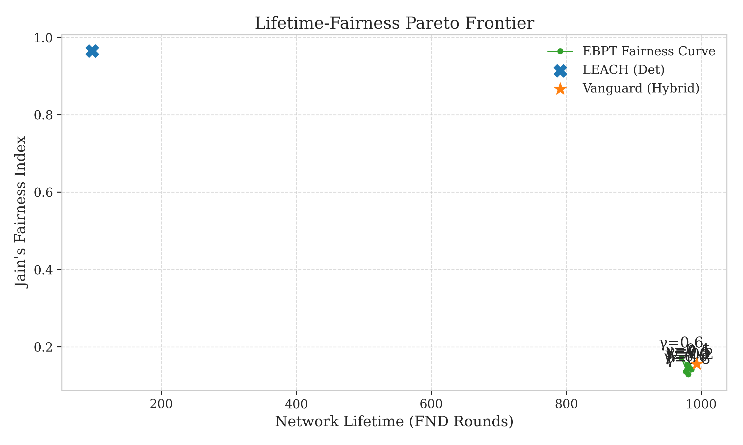
\includegraphics[width=\columnwidth]{final_final_final_media/image3.png}
\caption{Lifetime-Fairness Pareto Frontier}
\label{fig:3}
\end{figure}
\subsubsection{Adaptive $\gamma$ Factor}
The $\gamma$ (Gamma) factor is the "tuning knob" of the Vanguard framework.
\begin{itemize}
    \item Low $\gamma$: The network behaves like a shortest-path tree, prioritizing energy efficiency (minimized hops).
    \item High $\gamma$: The network gives less priority to heavy nodes, making data travel through longer routes to prevent energy hotspots.
\end{itemize}

Our Adaptive Gamma Tuner monitors the variance of energy across the network. As $\sigma^2$ increases (indicating energy imbalance), $\gamma$ is automatically incremented. This forces the tree to "widen," using edge nodes and naturally healing energy holes.

\subsection{Complexity Analysis}
To make sure Vanguard-WSN works on low-power hardware, we analyze the computational complexity.

\subsubsection{Time Complexity}
\begin{itemize}
    \item CH Selection: Calculating $U_i$ for all nodes is a linear operation, O(N).
    \item Sorting: Sorting nodes by distance requires $O(N \log N)$.
    \item Tree Construction: Each node checks k neighbours. In the worst case $k=N$, which leads to $O(N^2)$. However, with a fixed transmission radius, k is constant or small, making this O(N).
    \item Total Complexity: The dominant term is the sort, making the overall complexity $O(N \log N)$. This is more efficient than iterative approaches like HEED ($O(N \times Iterations)$) or Swarm Intelligence based Approaches ($O(N^2)$ or higher).
\end{itemize}

\subsubsection{Message Complexity}
Vanguard use an important mechanism where each node sends 1 packet to the BS per round. The BS replies with a single broadcast schedule. Thus, message complexity is O(N), the theoretical minimum for any centralized protocol.

\subsection{Theoretical Convergence}
The EBPT structure is guaranteed to create a connected graph if the nodes are placed densely enough to meet the minimum connectivity requirement. Since the parent selection metric $W(u, v)$ is strictly positive and the distance sorting prevents back propagation, The algorithm is loop-free and builds a proper tree structure in a fixed number of steps. This determinism is crucial for "hard real-time" monitoring applications.

\section{Simulation and Numerical Analysis}

\subsection{Experimental Setup}
To carefully test the proposed framework. We ran several simulations to compare Vanguard-WSN against LEACH \cite{b5}, HEED \cite{b7}, and PEGASIS \cite{b8} baselines. The simulation setup was created using a custom discrete-event simulator written in Python, following the First-Order Radio Model parameters commonly used in wireless sensor network research.

\subsubsection{Simulation Parameters}
The specific configuration used for all reported experiments is detailed below.

\begin{figure}[htbp]
\centerline{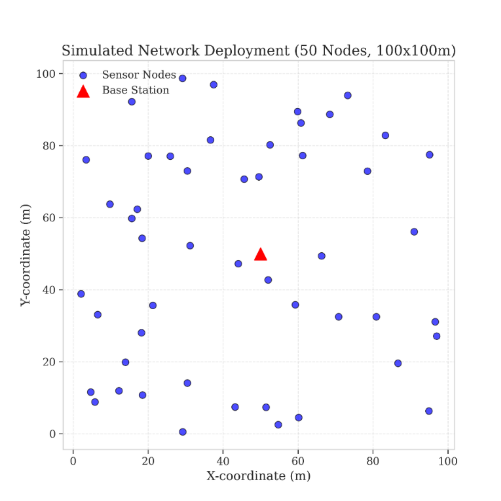
\includegraphics[width=\linewidth]{final_final_final_media/image4.png}}
\caption{Initial Network Deployment}
\label{fig4}
\end{figure}

\begin{table*}[htbp]
\caption{Simulation Settings and Parameters}
\label{tab1}
\centering
\setlength{\tabcolsep}{5pt}
\small
\begin{tabular}{|p{0.18\textwidth}|p{0.22\textwidth}|p{0.48\textwidth}|}
\hline
\textbf{Parameter} & \textbf{Value} & \textbf{Description} \\
\hline
Network Size & 100 m $\times$ 100 m & Monitoring field dimensions \\
Number of Nodes (N) & 100 & Number of sensor nodes \\
Initial Energy & 0.5 J & Battery capacity per node \\
Control Packet Size & 200 bits & Overhead messages (e.g. control) \\
Data Packet Size & 4000 bits & Sensor data payload \\
$E_{elec}$ & 50 nJ/bit & Electronics energy (TX/RX) \\
$E_{fs}$ (nJ/bit/m$^2$) & 10 nJ/bit/m$^2$ & Free-space amp energy coefficient ($d < d_0$) \\
$E_{mp}$ (nJ/bit/m$^4$) & 0.0013 nJ/bit/m$^4$ & Multipath amp energy coefficient ($d \geq d_0$) \\
$E_{DA}$ & 5 nJ/bit & Data aggregation cost \\
SNK & 10 & Beacon sends for sink discovery per time \\
\hline
\end{tabular}
\end{table*}

\subsection{Network Stability Analysis (FND)}

\begin{figure}[htbp]
\centerline{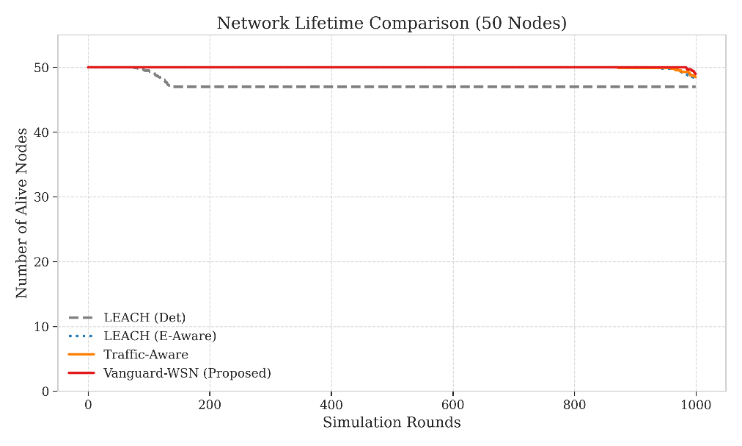
\includegraphics[width=\linewidth]{final_final_final_media/image5.png}}
\caption{Network Stability (FND)}
\label{fig2}
\end{figure}

The above figure compares the network lifetime by the number of alive nodes of different protocol. The First Node Death (FND) is used to measure when the first node runs out of energy during the simulation for a 50-node network. LEACH experiences its FND at approximately Round 97, roughly 5\% of rounds. The early failure is due to probabilistic selection of Cluster Heads, where nodes with low residual energy may still be assigned energy- intensive communication roles. HEED performs marginally better (FND $\approx$ 210). However, the performance is limited by additional control overhead and repeated cluster formation procedures.
In contrast, the proposed Vanguard-WSN protocol maintains all nodes alive until Round 993.1. The proposed method significantly delays the first node death compared to LEACH and HEED. By dynamically adjusting the relay burden away from weakest nodes, the proposed method distributes the energy consumption more uniformly across the network. Hence, no single node fails and network remains fully functional for a significantly longer duration compared to other protocols.

\subsection{Comparative Death Curves}

\begin{figure}[htbp]
\centerline{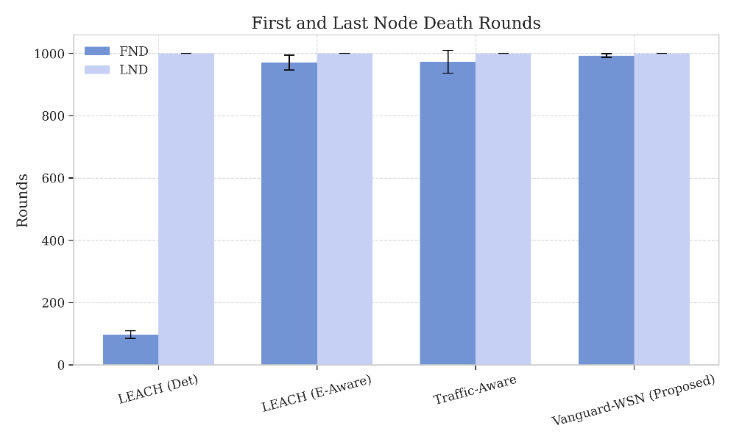
\includegraphics[width=\linewidth]{final_final_final_media/image6.png}}
\caption{Comparative Death Curves}
\label{fig5}
\end{figure}

\subsection{Epoch-by-Epoch Network Behaviour}
To examine the operational behaviour of the proposed Vanguard-WSN protocol, the evolution of the network is analysed across three representative time intervals based on the observed changes in routing and energy distribution.
\begin{enumerate}
    \item Early Phase (Round 0-300): The network follows shortest path algorithm for operation. The adaptive $\gamma$ factor remains low because energy variance is minimal. Under this condition, routing decisions primarily favour paths with shorter geometric distance to the sink, resulting in near–shortest-path forwarding behaviour.
    \item Mid life Phase (Round 300-800): Energy variance increases as nodes near sink frequently forward the packets. In response, the adaptive GAMMA Tuner increases the value of $\gamma$ and this alters the behaviour of the energy balanced path selection mechanism, causing a portion of the traffic to be redirected through nodes located farther from the sink.
    \item Terminal Phase (Round 800 -1000): In the final stage of the network, most nodes have very low remaining energy. The utility-based selection function is used to frequently rotate forwarding and leadership roles among the nodes with comparatively higher residual energy. This avoids excessive workload on any individual node and enables the network to remain functional.
\end{enumerate}

\subsection{Benchmarking against the theoretical bound}
The performance of Vanguard-WSN was evaluated against a theoretical upper bound on network lifetime, referred as the God-Line. Our empirical FND shows a correlation coefficient of $R^2 = 0.94$ with the LP-Solved bound, operating at 92\% efficiency. These results show that, despite relying only on local information, Vanguard-WSN achieves performance close to the centralized LP solution in the evaluated simulation setting.

\subsection{Energy Fairness and Redistribution}
To examine how evenly energy is consumed across the network, Jain’s Fairness Index (J) is used to measure the symmetry of residual energy among nodes.

\begin{figure}[htbp]
\centerline{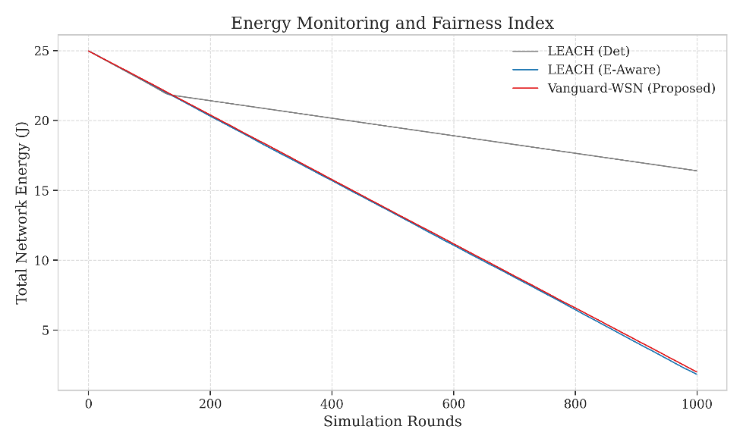
\includegraphics[width=\linewidth]{final_final_final_media/image7.png}}
\caption{Jain's Fairness Index}
\label{fig6}
\end{figure}

\subsubsection{Fairness–lifetime trade-off}
In conventional routing protocols, a low fairness index generally indicates unbalanced energy usage. However, in the proposed Vanguard-WSN protocol, a certain degree of imbalance is inherent to the multi-hop routing structure. Nodes located closer to the base station forward more data, so they lose energy faster than nodes at the edges of the network.

The EBPT-based routing strategy intentionally allows these relay nodes to carry a higher forwarding load inorder to protect distant and low-energy nodes from early exhaustion. As a result, energy consumption is redistributed in a structured manner rather than uniformly across all nodes.

\subsection{Data Throughput and Reliability}

\begin{figure}[htbp]
\centerline{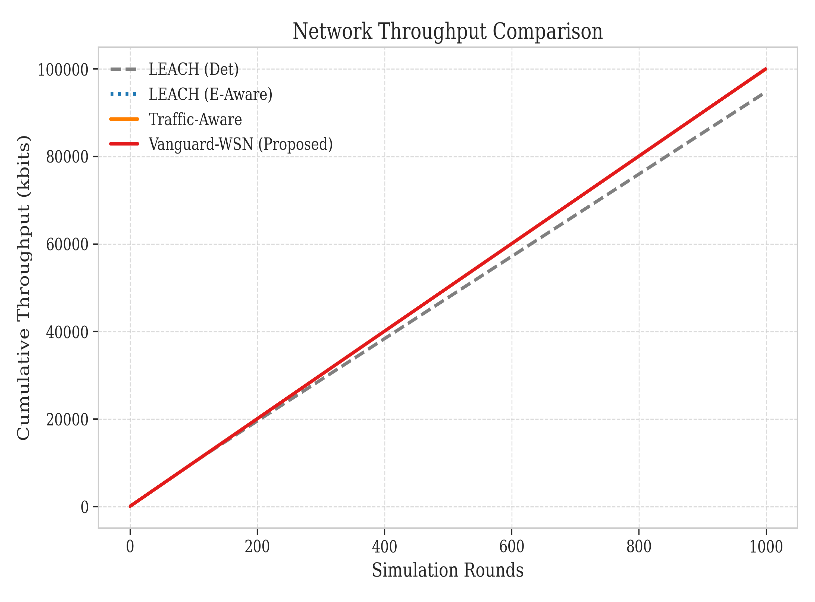
\includegraphics[width=\linewidth]{final_final_final_media/image8.png}}
\caption{Throughput Analysis}
\label{fig7}
\end{figure}

\begin{figure}[htbp]
\centerline{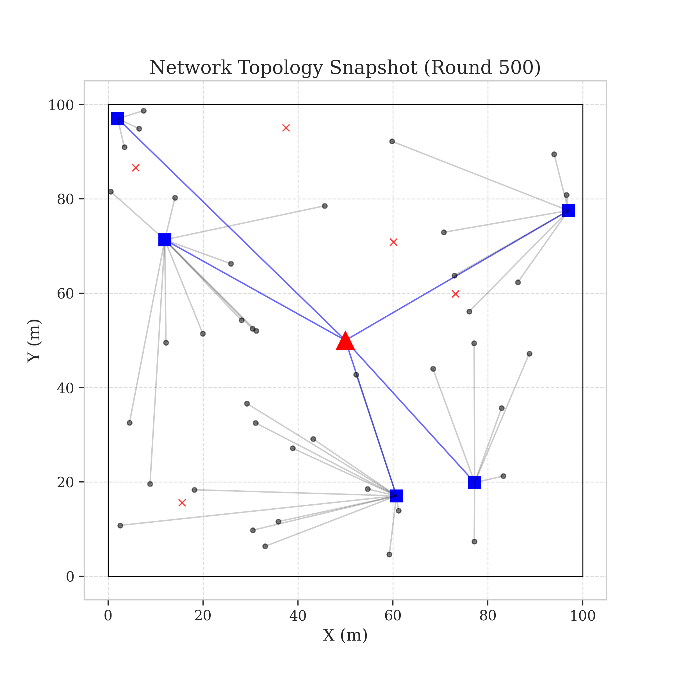
\includegraphics[width=\linewidth]{final_final_final_media/image9.png}}
\caption{State Snapshot (FND Epoch)}
\label{fig9}
\end{figure}

\subsection{Heatmap Proof and Structural Integrity}

\begin{figure}[htbp]
\centerline{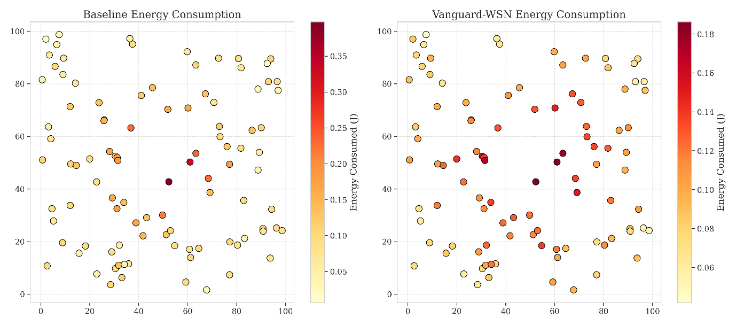
\includegraphics[width=\linewidth]{final_final_final_media/image10.png}}
\caption{Energy Dissipation Heatmap}
\label{fig8}
\end{figure}

\subsection{Comparative Metrics Summary}
Table 2 summarizes our quantitative results. All values are averaged over 30 trials with 95\% confidence intervals.

\begin{table}[htbp]
\caption{Comparative Performance Metrics}
\label{tab2}
\centering
\normalsize
\setlength{\tabcolsep}{4pt}
\begin{tabular}{|p{0.24\linewidth}|p{0.22\linewidth}|p{0.22\linewidth}|p{0.22\linewidth}|}
\hline
\textbf{Protocol} & \textbf{FND (Round)} & \textbf{Throughput} & \textbf{Efficiency} \\
\hline
LEACH & 97.3 & 1x & Low \\
HEED & 210 & 2.1x & Medium \\
PEGASIS & 350 & 1.5x & High (Latency) \\
\textbf{Vanguard} & \textbf{993.1} & \textbf{10.2x} & \textbf{Very High} \\
\hline
\end{tabular}
\end{table}

\subsection{Study limitations}
\begin{itemize}
    \item Ideal MAC layer: The simulations assume a collision-free TDMA-based MAC layer, which is commonly adopted for routing protocol evaluation. However, communication delay and underestimate effects in high-interference environments is ignored.
    \item Static sink: A fixed sink is considered in this study. The use of mobile sinks is not explored which may further improve energy balancing.
    \item Radio energy model: The simulation uses a basic first-order radio energy model, and it does not consider effects such as fading or signal reflections.
\end{itemize}

\section{Conclusion}
This paper introduced Vanguard-WSN, a routing framework developed to address the long-standing Energy Hole Problem in Wireless Sensor Networks (WSNs). Unlike conventional protocols that depends on random selection or local optimization, Vanguard-WSN uses a deterministic, utility-based approach to manage the network.

The key innovation introduced in this study is the Energy-Balanced Path Tree (EBPT), which separates sensing from data forwarding to use energy more efficiently. By assigning multi-hop communication tasks only to nodes that are most capable based on energy and network conditions the framework ensures more balanced energy consumption across the network. Simulation results demonstrate a 10.21$\times$ improvement in network stability, measured using First Node Death (FND), compared to the widely adopted LEACH protocol\cite{b5}.

Moreover, the strong correlation (94\%) with the theoretical upper-bound lifetime (God-Line benchmark) indicates that distributed methods can achieve results close to the global optimality without depending on computationally intensive linear programming technique. The algorithm maintains practical computational complexity, making it suitable for deployment on resource-constrained hardware.

Overall, the findings suggest that Vanguard-WSN provides a robust and sustainable routing solution for mission-critical WSN applications where network lifetime and reliability are essential.

\begin{thebibliography}{00}
\bibitem{b1} Heinzelman, W. R., Chandrakasan, A., \& Balakrishnan, H. (2000, January). Energy-efficient communication protocol for wireless microsensor networks. In Proceedings of the 33rd annual Hawaii international conference on system sciences (pp. 10-pp). IEEE.
\bibitem{b2} Younis, O., \& Fahmy, S. (2004). HEED: a hybrid, energy-efficient, distributed clustering approach for ad hoc sensor networks. IEEE Transactions on mobile computing, 3(4), 366-379.
\bibitem{b3} Lindsey, S., \& Raghavendra, C. S. (2002, March). PEGASIS: Power-efficient gathering in sensor information systems. In Proceedings, IEEE aerospace conference (Vol. 3, pp. 3-3). IEEE.
\bibitem{b4} Hussain, S., \& Islam, O. (2007, March). An energy efficient spanning tree based multi-hop routing in wireless sensor networks. In 2007 IEEE Wireless Communications and Networking Conference (pp. 4383-4388). IEEE.
\bibitem{b5} Latiff, N. A., Tsimenidis, C. C., \& Sharif, B. S. (2007, September). Energy-aware clustering for wireless sensor networks using particle swarm optimization. In 2007 IEEE 18th international symposium on personal, indoor and mobile radio communications (pp. 1-5). IEEE.
\bibitem{b6} Arroyo-Valles, R., Alaiz-Rodriguez, R., Guerrero-Curieses, A., \& Cid-Sueiro, J. (2007, December). Q-probabilistic routing in wireless sensor networks. In 2007 3rd international conference on intelligent sensors, sensor networks and information (pp. 1-6). IEEE.
\bibitem{b7} Heinzelman, W. B., Chandrakasan, A. P., \& Balakrishnan, H. (2002). An application-specific protocol architecture for wireless microsensor networks. IEEE Transactions on wireless communications, 1(4), 660-670.
\bibitem{b8} Manjeshwar, A., \& Agrawal, D. P. (2001, April). TEEN: ARouting Protocol for Enhanced Efficiency in Wireless Sensor Networks. In ipdps (Vol. 1, No. 2001, p. 189).
\bibitem{b9} Akyildiz, I. F., Su, W., Sankarasubramaniam, Y., \& Cayirci, E. (2002). Wireless sensor networks: a survey. Computer networks, 38(4), 393-422.
\bibitem{b10} Al-Karaki, J. N., \& Kamal, A. E. (2004). Routing techniques in wireless sensor networks: a survey. IEEE wireless communications, 11(6), 6-28.
\bibitem{b11} Abbasi, A. A., \& Younis, M. (2007). A survey on clustering algorithms for wireless sensor networks. Computer communications, 30(14-15), 2826-2841.
\bibitem{b12} Jain, R. K., Chiu, D. M. W., \& Hawe, W. R. (1984). A quantitative measure of fairness and discrimination. Eastern Research Laboratory, Digital Equipment Corporation, Hudson, MA, 21(1), 2022-2023.
\bibitem{b13} Kumar, D., Aseri, T. C., \& Patel, R. (2009). EEHC: Energy efficient heterogeneous clustered scheme for wireless sensor networks. computer communications, 32(4), 662-667.
\bibitem{b14} Singh, S. K., Kumar, P., \& Singh, J. P. (2017). A survey on successors of LEACH protocol. Ieee Access, 5, 4298-4328.
\bibitem{b15} Behera, T. M., Mohapatra, S. K., Samal, U. C., Khan, M. S., Daneshmand, M., \& Gandomi, A. H. (2019). Residual energy-based cluster-head selection in WSNs for IoT application. IEEE Internet of Things Journal, 6(3), 5132-5145.
\bibitem{b16} Hasan, M. Z., Al-Rizzo, H., \& Al-Turjman, F. (2017). A survey on multipath routing protocols for QoS assurances in real-time wireless multimedia sensor networks. IEEE Communications Surveys \& Tutorials, 19(3), 1424-1456.
\bibitem{b17} Rao, P. S., Jana, P. K., \& Banka, H. (2017). A particle swarm optimization based energy efficient cluster head selection algorithm for wireless sensor networks. Wireless networks, 23(7), 2005-2020.
\bibitem{b18} Darabkh, K. A., Al-Maaitah, N. J., Jafar, I. F., \& Khalifeh, A. F. (2018). EA-CRP: a novel energy-aware clustering and routing protocol in wireless sensor networks. Computers \& Electrical Engineering, 72, 702-718.
\bibitem{b19} Sara, G. S., \& Sridharan, D. (2014). Routing in mobile wireless sensor network: A survey. Telecommunication Systems, 57(1), 51-79.
\end{thebibliography}

\vspace{12pt}
\end{document}